\documentclass[a4paper]{article}
\usepackage[
    top=2.5cm,
    bottom=2.5cm,
    left=3cm,
    right=3cm
]{geometry}
\usepackage{amsmath}
\usepackage{amsfonts}
\usepackage{physics}
\usepackage{graphicx}
\usepackage{wasysym}
\usepackage{subcaption}
\usepackage[backend=bibtex8]{biblatex}
\usepackage[linkcolor=blue, colorlinks=true]{hyperref}

\addbibresource{references.bib}

\title{String breaking in $\mathbb{Z}_2$-Higgs model on IBM machines \\[15pt]
       \large Project notes}
\author{Jesús Cobos Jiménez}

\begin{document}

\maketitle

\section{Objective}

This project goal is to use IBM's machines to simulate some physical model. Our intention is to push the capabilities of the current devices to their limit and obtain a simulation that is \textit{at least} qualitatively correct. If possible, we will try to also obtain quantitative insights, but we have to be conscious of the devices' limitations. The harder the target system is to simulate, the better. We do not plan on claiming \textit{quantum advantage}, but we would like the resulting simulation to be non-trivial to perform on a classical machine. This reasoning suggests that we should try to simulate some dynamical effect. Also, the considered model must be in close correspondence with the IBM machines themselves in terms of geometry and nature of the degrees of freedom. Considering the previous premises and our own expertise, we have opted to simulate the string-breaking phenomenon in the $\mathbb{Z}_2$-Higgs model in $(2+1)$ dimensions in a hexagonal lattice. Fig.~\ref{fig:roadmap} shows our roadmap for the project. We are currently moving to 2D lattices.

\begin{figure}[!ht]
    \centering
    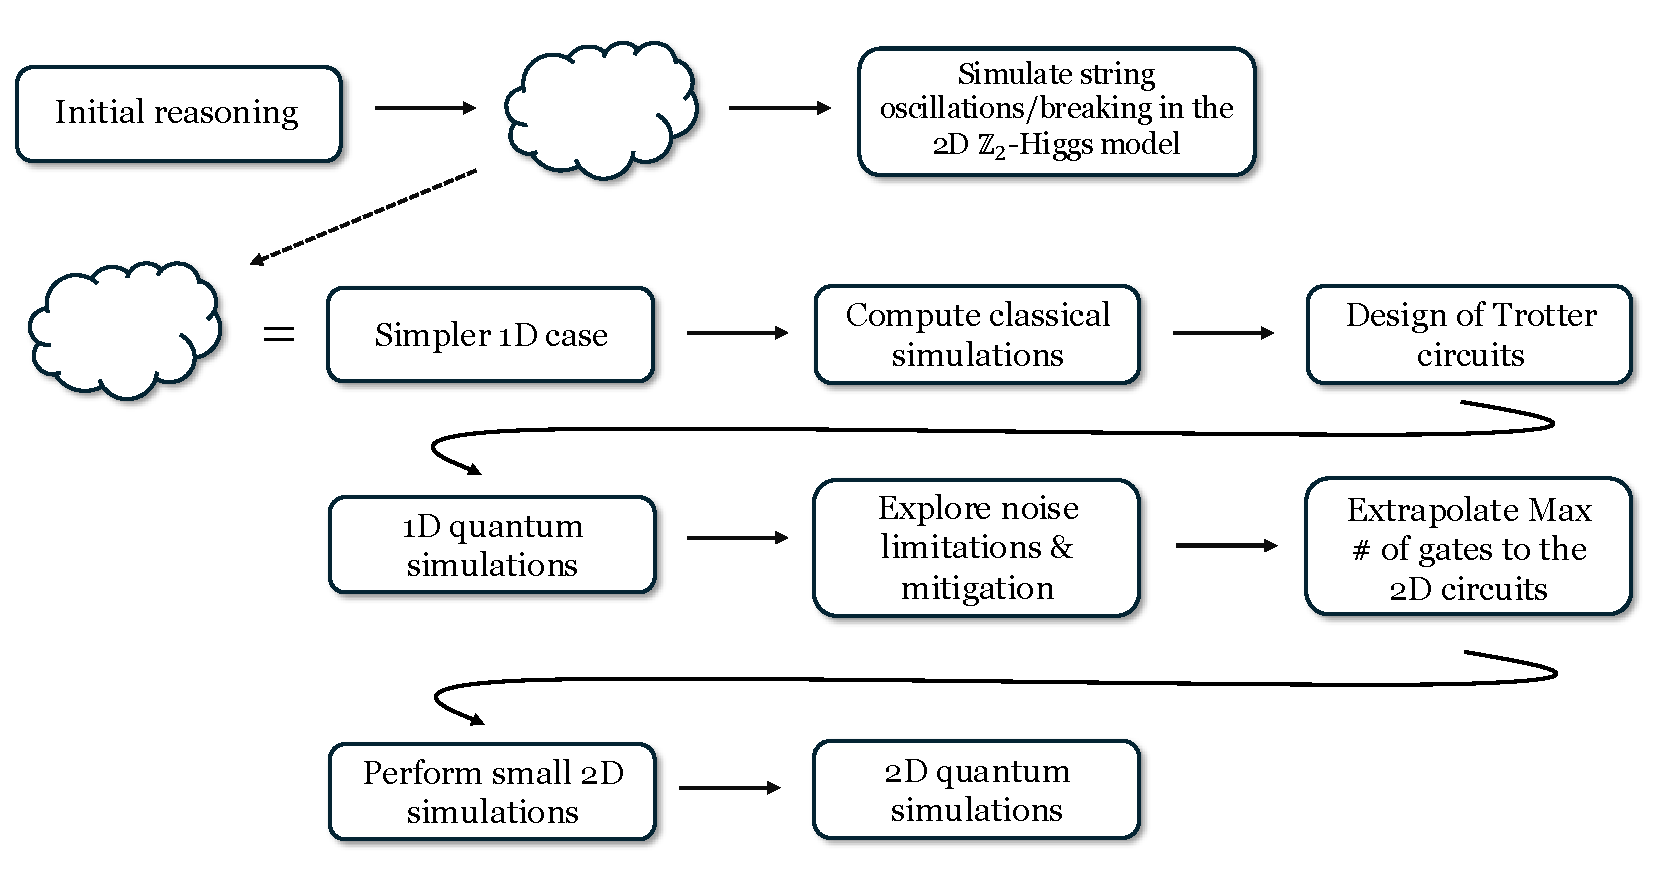
\includegraphics[width=0.9\textwidth]{Roadmap.pdf}
    \caption{Project's Roadmap}
    \label{fig:roadmap}
\end{figure}

\section{The model}

The $\mathbb{Z}_2$-Higgs model is a lattice gauge theory in $(2+1)$ dimensions with qubit matter and gauge degrees of freedom. The Hamiltonian for this LTG is the following:
%
\begin{equation}
    H = \underbrace{-\frac{J}{\lambda} \sum_{n} \tau_{n}^z}_{\text{Mass term}} - \underbrace{\frac{h}{\lambda} \sum_{(n, v)} \sigma_{n, v}^{z}}_{\text{Electric energy}} - \underbrace{\sum_{n, v} \tau_{n + v}^x \sigma_{(n, v)}^x \tau_{n}^x}_{\text{Matter-gauge interaction}} - \underbrace{\frac{\beta}{\lambda} \sum_{n} \prod_{m, v \in \hexagon_n} \sigma_{(m, v)}^z}_{\text{Magnetic energy}}
    \label{eq:hamiltonian}
\end{equation}
%
Where $\tau$, $\sigma$ are Pauli matrices referring to the matter and gauge degrees of freedom respectively, $n, m$ denote sites on the hexagonal lattice and $v$ unit lattice vectors. As usual, matter lives in the nodes of the lattices while gauge d.o.f. live on the links as shown in Fig.~\ref{fig:lattice}. The Hamiltonian for the simpler $(1+1)$ case remains the same with the magnetic energy is removed.

\begin{figure}
    \centering
    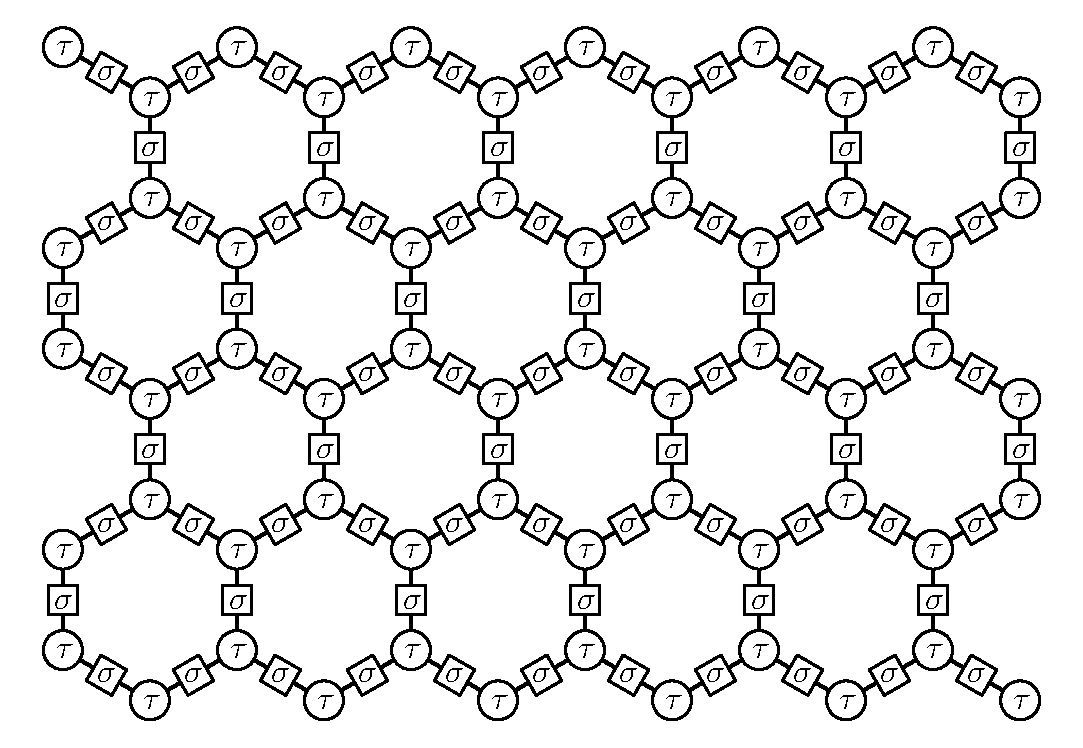
\includegraphics[width=0.6\textwidth]{honeycomb.pdf}
    \caption{$\mathbb{Z}_2$-Higgs model in the honeycomb lattice}
    \label{fig:lattice}
\end{figure}

As it is always the case in lattice gauge theories, there is a set of local symmetries acting in every node of the lattice. In this case, the gauge symmetry operators are the following:
%
\begin{equation}
    G_n = \tau_n^z \prod_{v \in \ell_n} \sigma_{(n, v)}^z \hspace{2cm} \left[G_n, H\right] = 0 \hspace{0.5cm} \forall n
    \label{eq:gauge}
\end{equation}
%
with $\ell_n$ denoting the directions of the links connected to node $n$. Since gauge symmetries commute with the Hamiltonian of the system, they are a constant of motion. They divide the complete Hilbert space of the system into sectors corresponding to states with different eigenvalues
%
\begin{equation}
    G_n \ket{\psi} = \pm \ket{\psi},
\end{equation}
%
which are related to the absence ($+$) or presence ($-$) of non-dynamical background charge in site $n$ of the lattice. Usually, we call \textit{physical states} those fulfilling condition $G_n\ket{\psi} = \ket{\psi}\; \forall n$.

Due to the difficulty of implementing plaquette operators in the IBM machines, we will restrict to the confined regime ($\beta \sim 0$). Note that third order perturbation theory on the matter-gauge interaction yields the plaquette operator because the matter terms cancel out due to the fact that $(\tau^z)^2 = 1$ and each matter site is connected to three links. This should be enough to observe string oscillations and string breaking in the correct regime.

\section{Trotter circuits}

\subsection{(1+1) case}

The study of the simpler (1+1) $\mathbb{Z}_2$-Higgs chain is interesting because the circuits that simulate the dynamics in both this and the $(2+1)$ case will have a similar structure. We use the $(1+1)$ case as a classically simulable benchmark to address the effect of noise in the devices and set the basics to the $(2+1)$ case.

To simulate the dynamics of the $\mathbb{Z}_2$-Higgs model we perform a trotterized time evolution. We opt for a second order Trotter expansion
%
\begin{equation}
    U(t) = e^{-i H t} = \lim_{N \to \infty}\left( e^{-i H_M t/2N} e^{-i H_I t/N} e^{-i H_M t/2N} \right)^N.
    \label{eq:trotter}
\end{equation}
%
With $H_M$ the 1-local terms and $H_I$ the higher weight terms in Hamiltonian \eqref{eq:hamiltonian}. Our choice is motivated by the fact that, although higher order Trotter expansions are more precise, they lead to longer circuits. We want to minimize circuit depth because that is the limiting factor in real hardware. The second order Trotter expansion is equivalent terms of two qubit depth as the first order so using it is free complexity-wise.

Fig.~\ref{fig:circs}(a) shows the straightforward implementation of a single Trotter step of expansion \eqref{eq:trotter}. At first, we opted to do an alternating implementation of the time evolution operators of $H_I$ terms. Simple CNOT swapping yields the denser circuit in Fig. \ref{fig:circs}(b). The single qubit rotations at the beginning and end of the circuit implement the time evolution operators of the local terms. The train of CNOTs around the $R_x(\theta)$ rotation implements the time evolution operator for the matter-gauge interaction terms.

\begin{figure}
    \centering
    \begin{subfigure}[bl]{0.3\textwidth}
        \centering
        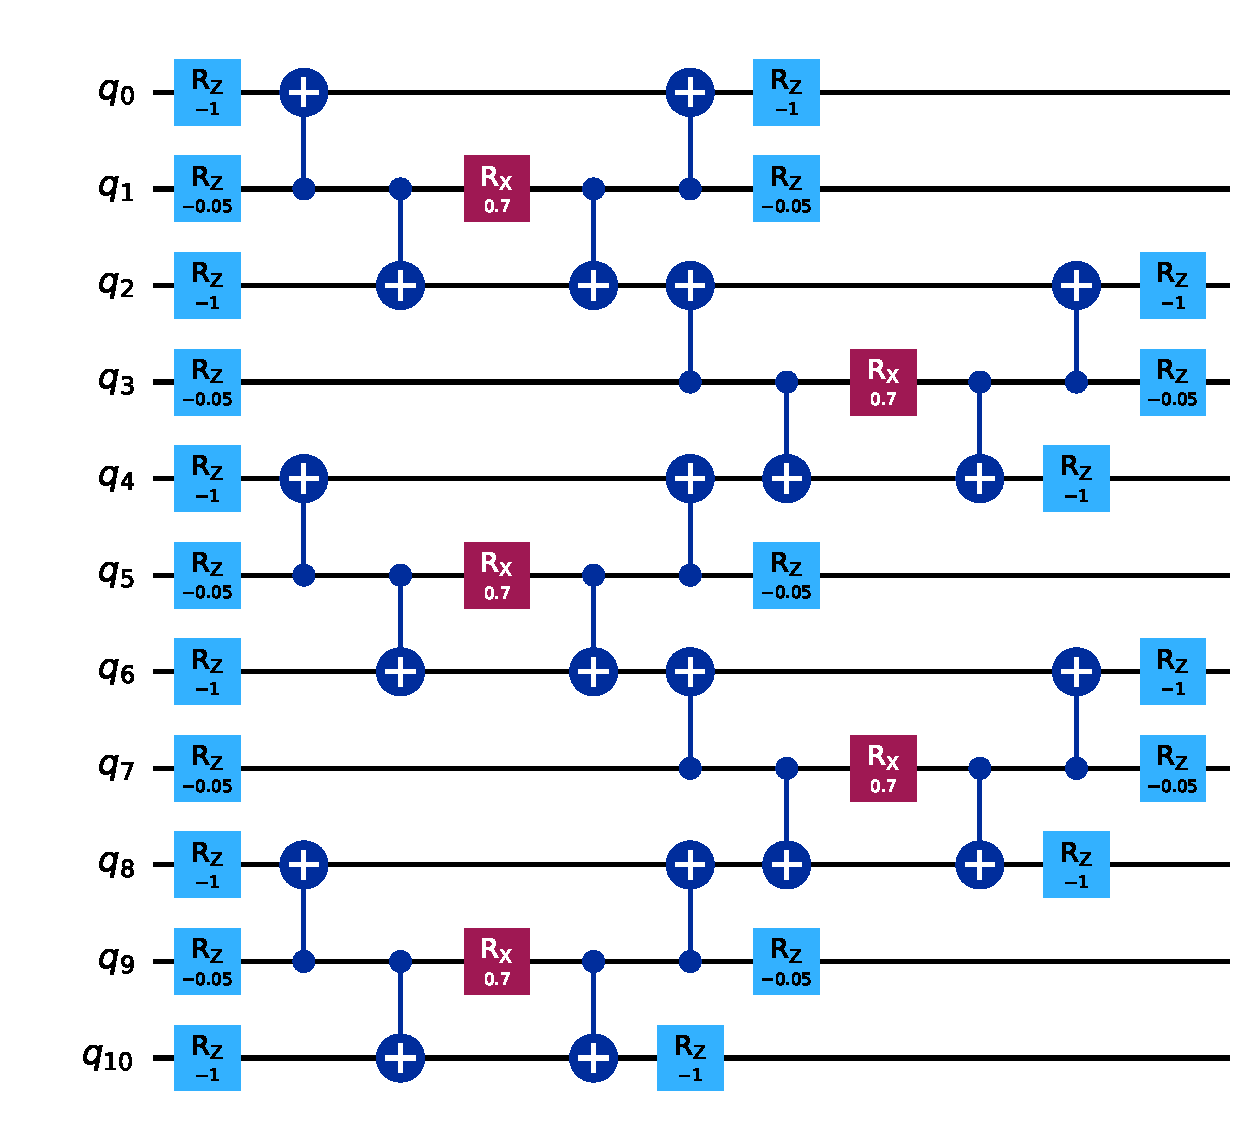
\includegraphics[width=0.99\textwidth]{second_order_trotter_old.pdf}
        \caption{Straightforward implementation}
    \end{subfigure}
    \begin{subfigure}[bl]{0.3\textwidth}
        \centering
        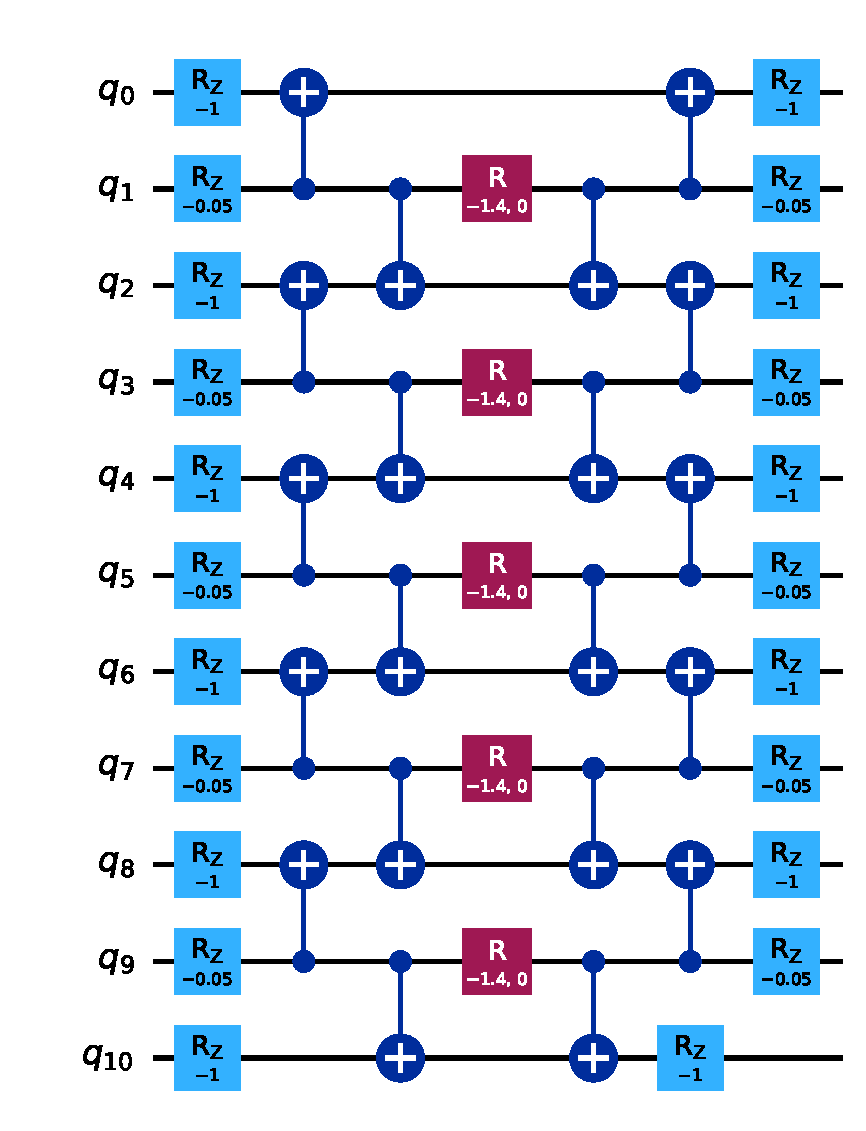
\includegraphics[width=0.72\textwidth]{second_order_trotter.pdf}
        \caption{Dense implementation}
    \end{subfigure}
    \begin{subfigure}[position]{0.3\textwidth}
        \centering
        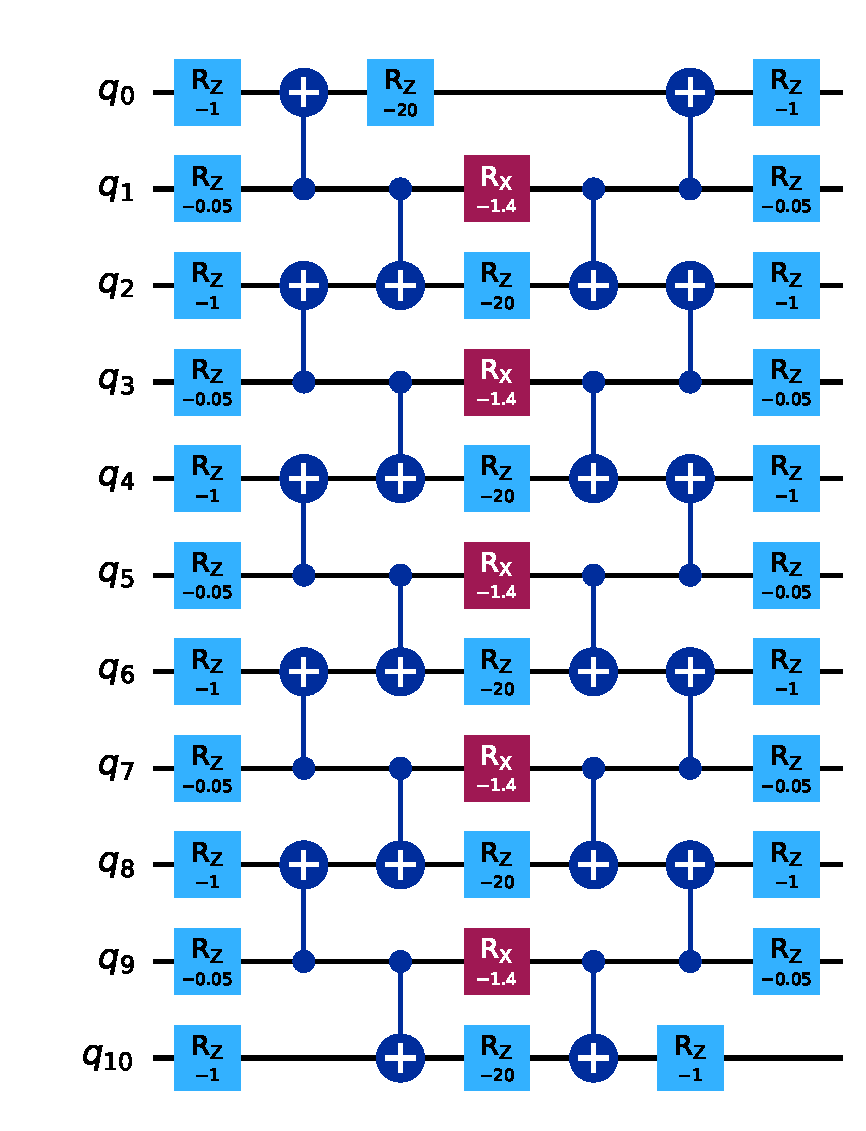
\includegraphics[width=0.72\textwidth]{second_order_trotter_gauge.pdf}
        \caption{Gauge Dynamical decoupling}
    \end{subfigure}
    \caption{Trotter layer implementation.}
    \label{fig:circs}
\end{figure}

We are currently exploring the addition of extra terms to the Hamiltonian corresponding to a sum of gauge operators
%
\begin{equation}
    \tilde{H} = H + \sum_n G_n.
    \label{eq:hamiltonian_gauge}
\end{equation}
%
The inclusion of gauge symmetry operators into the Hamiltonian itself leaves the dynamics of the system invariant because of their commutation relation \eqref{eq:gauge}, however in the presence of hardware noise, they will induce a phase into \textit{unphysical states} that suppresses them similarly to dynamical decoupling. Figure \ref{fig:circs}(c) shows one Trotter step of the evolution generated by Hamiltonian \eqref{eq:hamiltonian_gauge}.

\subsection{(2+1) case}

We must implement the circuits for the time evolution in the $(2+1)$ dimensional case. The structure of the circuits is presumably similar to the $(1+1)$ case, but in principle will be less dense because now, each matter link is connected to three links. If one uses the straightforward implementation (Fig.~\ref{fig:circs}(a)) as basis for simplifications, three alternating rows of interaction time evolution operators will appear. It may not be possible to combine the third one into a dense layer of operations as in Fig.~\ref{fig:circs}(b) because the targets and control of CNOTs will overlap. However, we must still explore what is the shortest circuit that we can come up with. Since we should look for dense circuits because idle qubits are more prone to errors in hardware, another ouption is to introduce gauge time evolution operators in the remaining gaps. The steps to be followed to design the circuits in the $(2+1)$ case are the following (open to debate):

\begin{enumerate}
    \item Design a general mapping between d.o.f. in the simulated lattice and physical qubits in IBM devices. We will refer to the size of the lattice with the number of plaquettes that it contains in the horizontal $P_x$ and vertical $P_y$ directions. For the mapping into the device, we should indicate where is the top left plaquette of our lattice placed on the device ($D_x$, $D_y$). With this input, we must write a Python function that takes $P_x$, $P_y$ and ($D_x$, $D_y$) as input and returns a list of physical qubits and three sets of node-link-node triples of qubits such as each set contains unique links.
    \item Write a Python function that takes the three previous node-link-node triples sets and returns the desired circuit with its proper layout. These sets define the order of the operations in the circuits.
\end{enumerate}

\subsection{Setting the number of Trotter layers}

When simulating trotterized temporal evolutions in quantum devices there is a trade-off between the error arising from the finite number of trotter layers and the accumulation of noise-induced errors. For certain time of evolution $t$, we estimate the optimal the number of Trotter layers $N_L$ by equating the asymptotic Trotter error for the second order expansion
%
\begin{equation}
    \varepsilon \sim (t/N_L)^3,
    \label{eq:trotter_error}
\end{equation}
%
to the success probability of a circuit execution that is related to the error per layered gate (EPLG) metric provided by IBM \cite{mckay2023benchmarkingquantumprocessorperformance}
%
\begin{equation}
    P(\mathrm{Success}) = 1 - (1-\text{EPGL})^{4 N_L}.
    \label{eq:success_probability}
\end{equation}
%
The curves defined by Eqs.~(\ref{eq:trotter_error}, \ref{eq:success_probability}) intersect at some point which defines the optimal number of Trotter layers as in Fig.~\ref{fig:optimal_layers}.

\begin{figure}
    \centering
    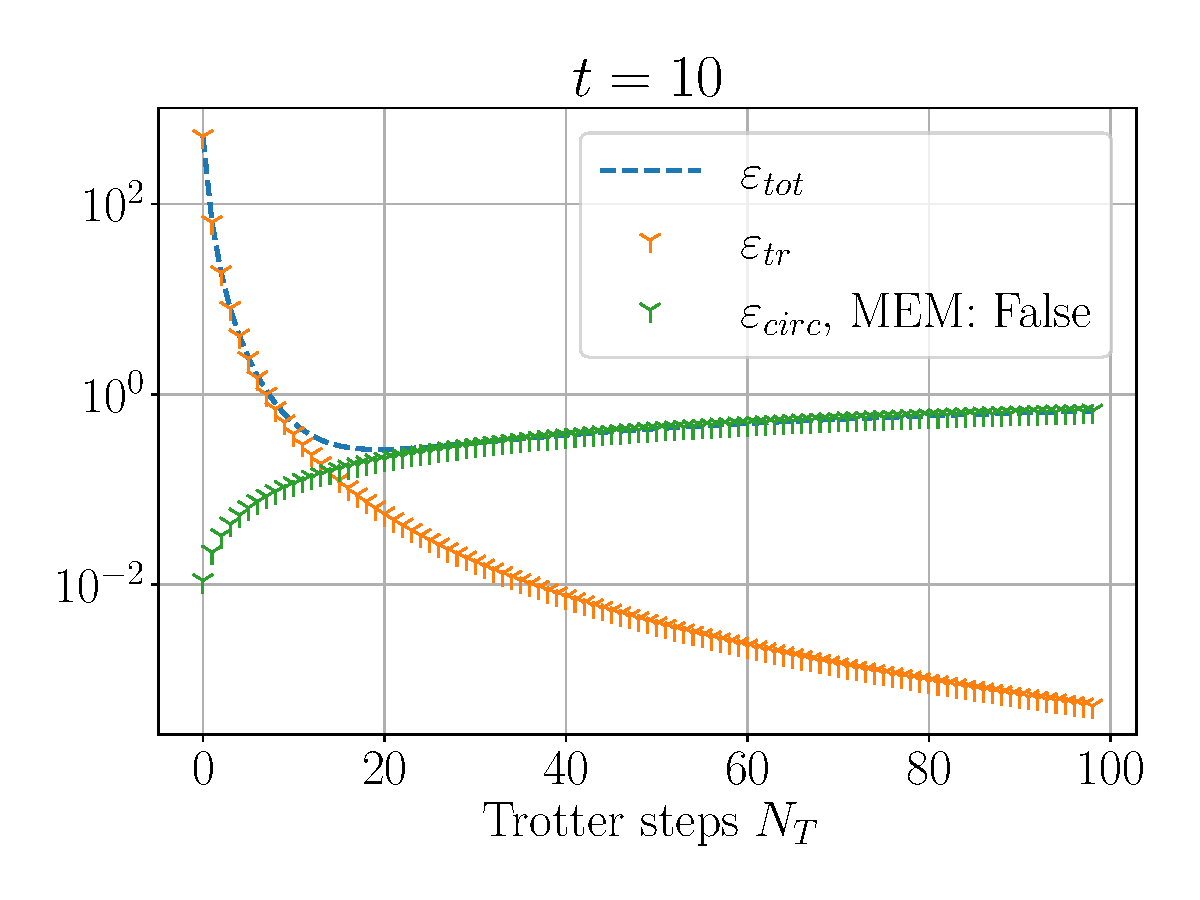
\includegraphics[width=0.55\textwidth]{optimal_trotter.pdf}
    \caption{Success probability and trotter error curves.}
    \label{fig:optimal_layers}
\end{figure}

\section{Noise mitigation}

Qiskit offers a suite of noise mitigation techniques of which we make use to reduce the effect of circuit error and actually get signal. We currently use:

\begin{itemize}
    \item Twirled readout error extinction: Add random Paulis before measurement to turn noise into dephasing channel.
    \item Dynamical decoupling: Add pulses to idle qubits to counteract dephasing noise.
    \item Pauli twirling: Add random Paulis before and after gates to turn noise into dephasing channel.
    \item ZNE: Induce more noise into circuits by repeating them in a compute-uncompute fashion and perform extrapolation to the no noise regime.
\end{itemize}

We also use the gauge symmetries to perform postselection and discard the circuit repetitions in which we know for certain an error has occurred. The ratio of discarded to total samples in terms of the 2-qubit depth of circuits (increasing evolution time) for a small $L=8$ chain is shown in Fig.~\ref{fig:postselection_samples}.

\begin{figure}
    \centering
    \hspace{-1cm}
    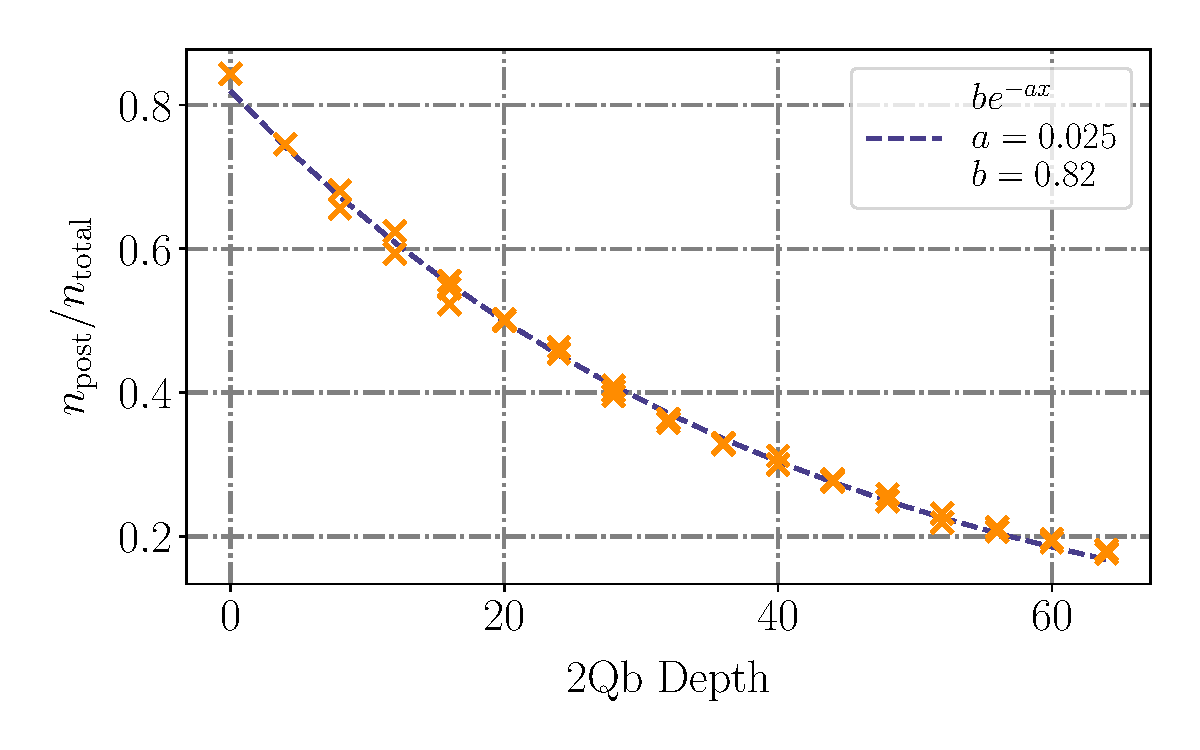
\includegraphics[width=0.6\textwidth]{postselected_samples.pdf}
    \caption{Ratio of discarded to total samples in a small $L=8$ chain for increasing 2-qubit circuit depth.}
    \label{fig:postselection_samples}
\end{figure}

\section{Results}

\subsection{(1+1) case}

Figure FIG shows the dynamics of the mean occupation
%
\begin{equation}
    N_n = \frac{1 - \langle \sigma_n^z \rangle}{2}
\end{equation}
%
of matter and gauge sites in chains of different length for an initial state consisting in a string of length $L_s = 1$ centered in the middle of the chain. In all cases, the constant in the Hamiltonian are the following: $J = 1$, $h = 0.01$, $\lambda = 0.7$. The maximum time of evolution is $t = 8$.

\begin{figure}[!ht]
    \centering
    \begin{subfigure}[l]{0.4\textwidth}
        \centering
        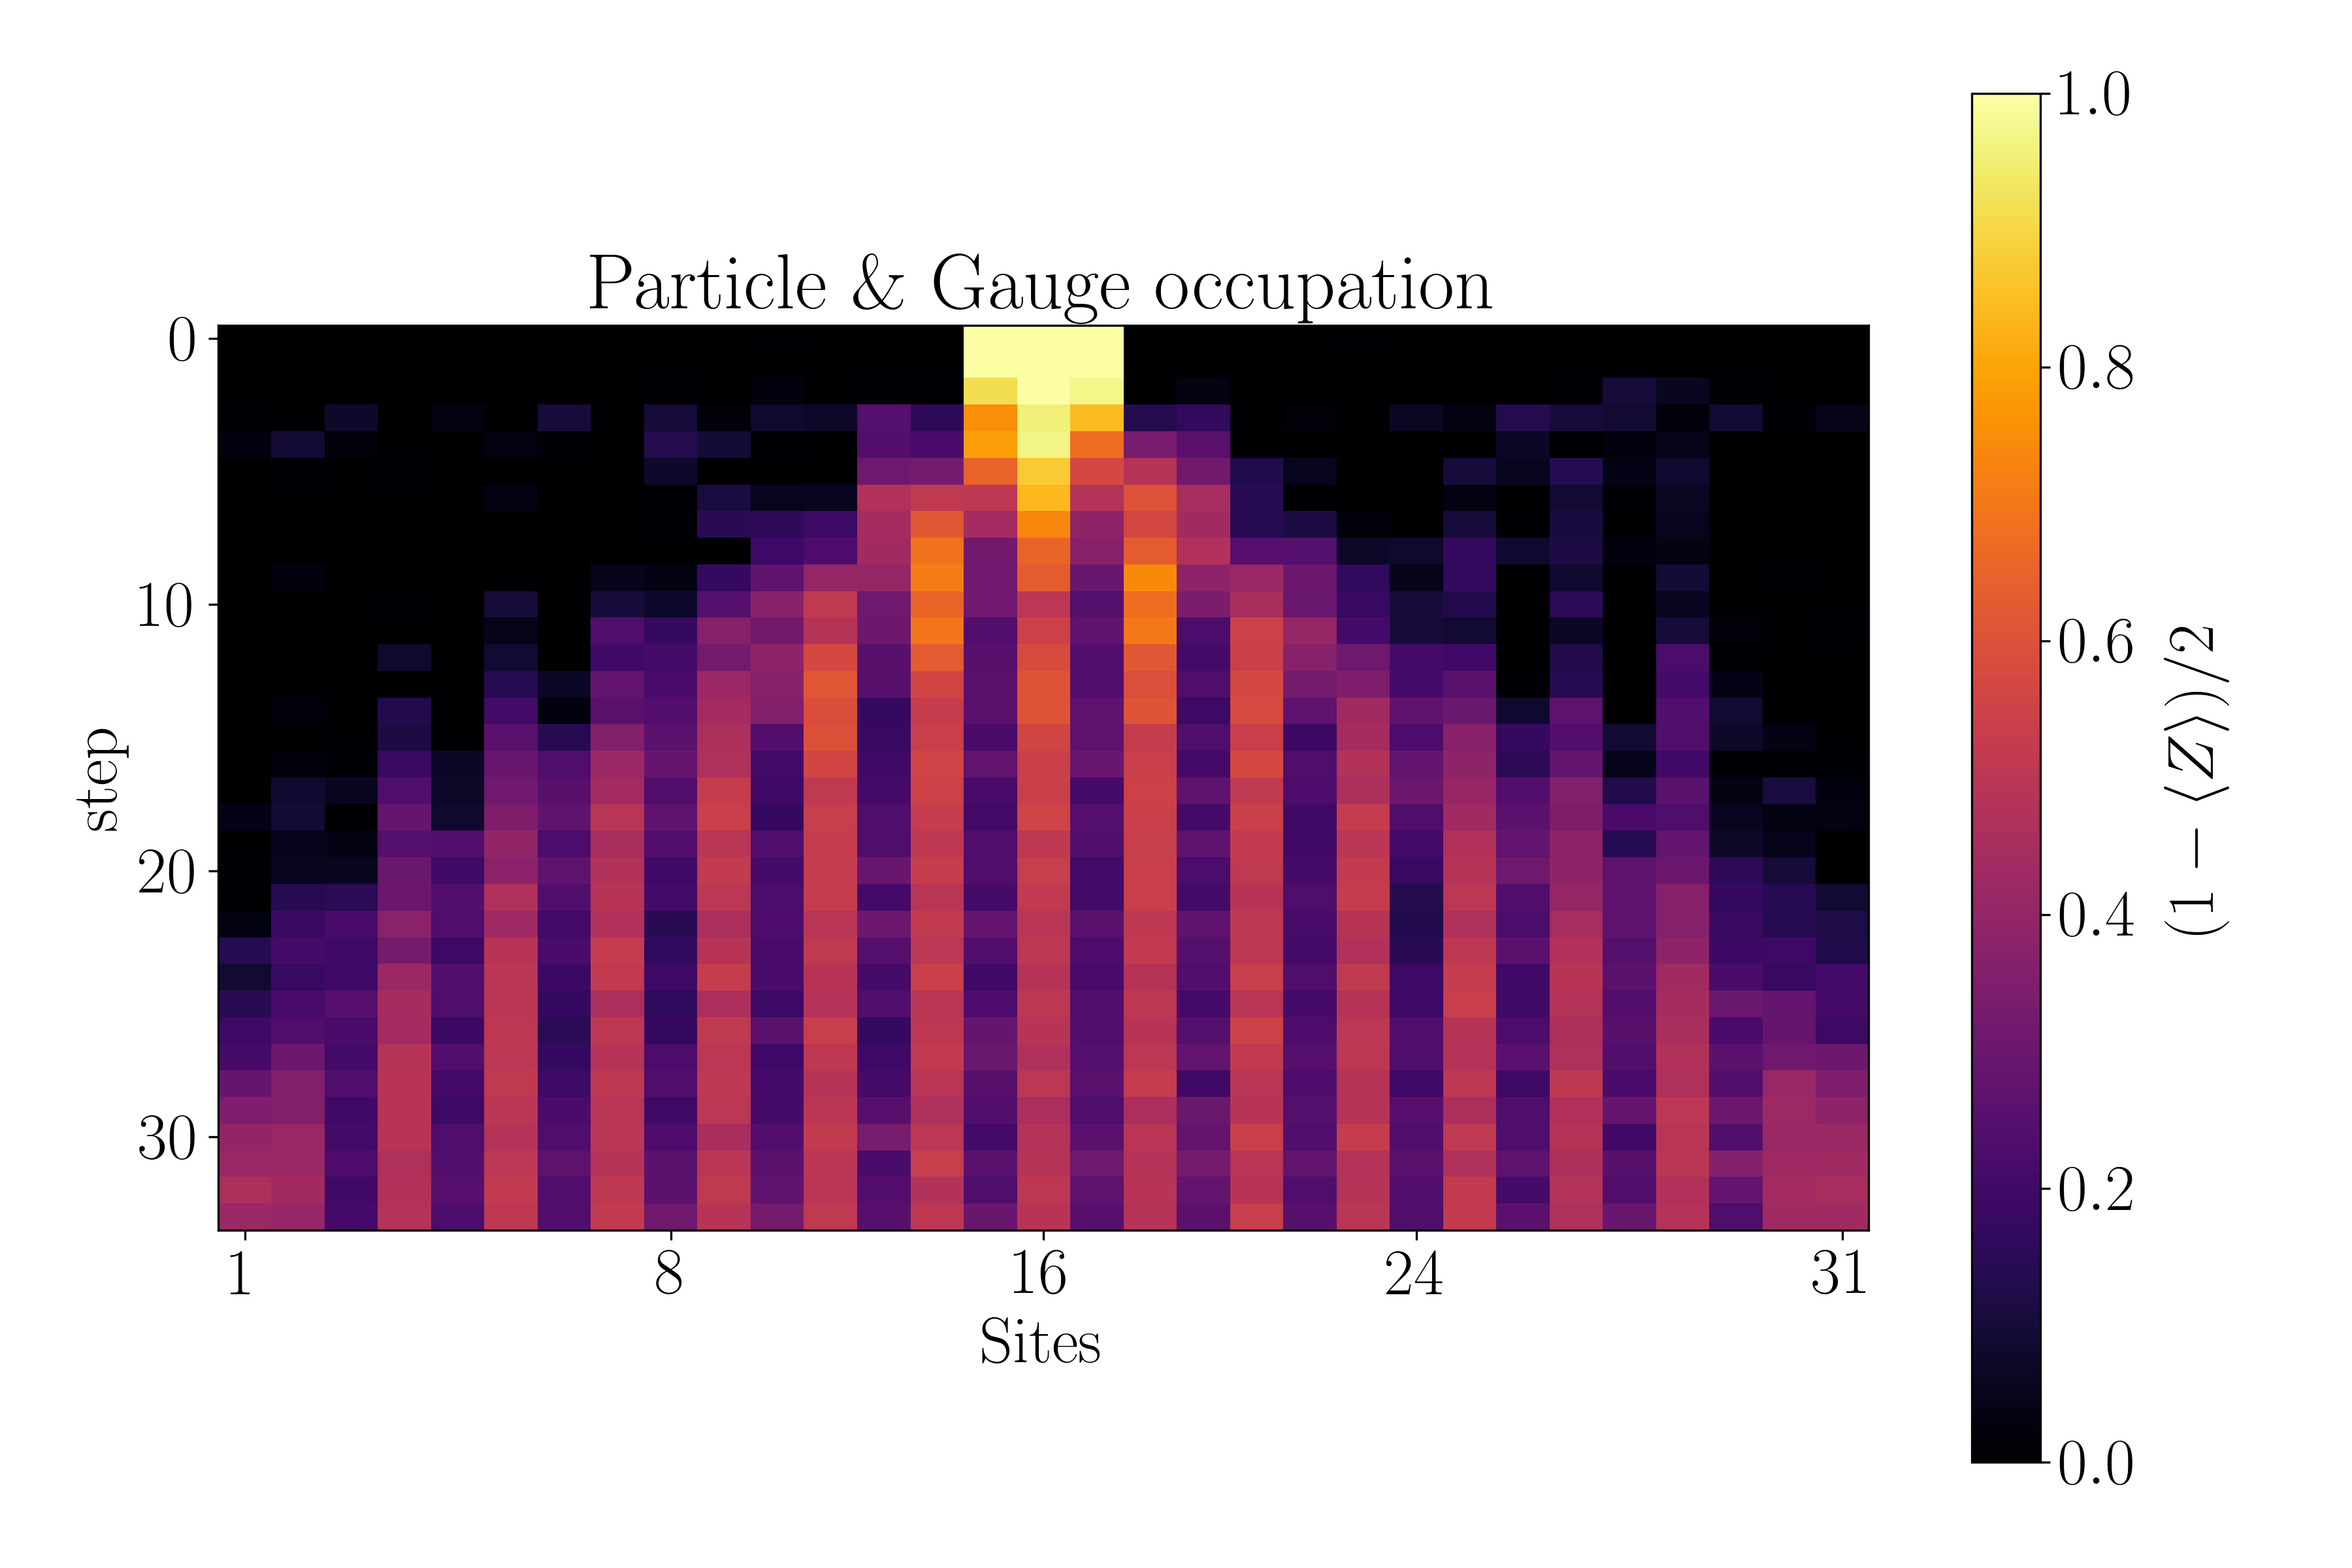
\includegraphics[width=\textwidth]{Results figs/hardware_z2pairquench_maxt_8_steps_35_L_16_J_1.0000_h_0.0500_lamb_0.7000_g_None_pp_7_pl_1_zne_True_linear_1-1.2-1.5_mm_True_dc_XY4_pt_True_xbasis_False.png}
        \caption{$L = 16$}
    \end{subfigure}
    \begin{subfigure}[l]{0.58\textwidth}
        \centering
        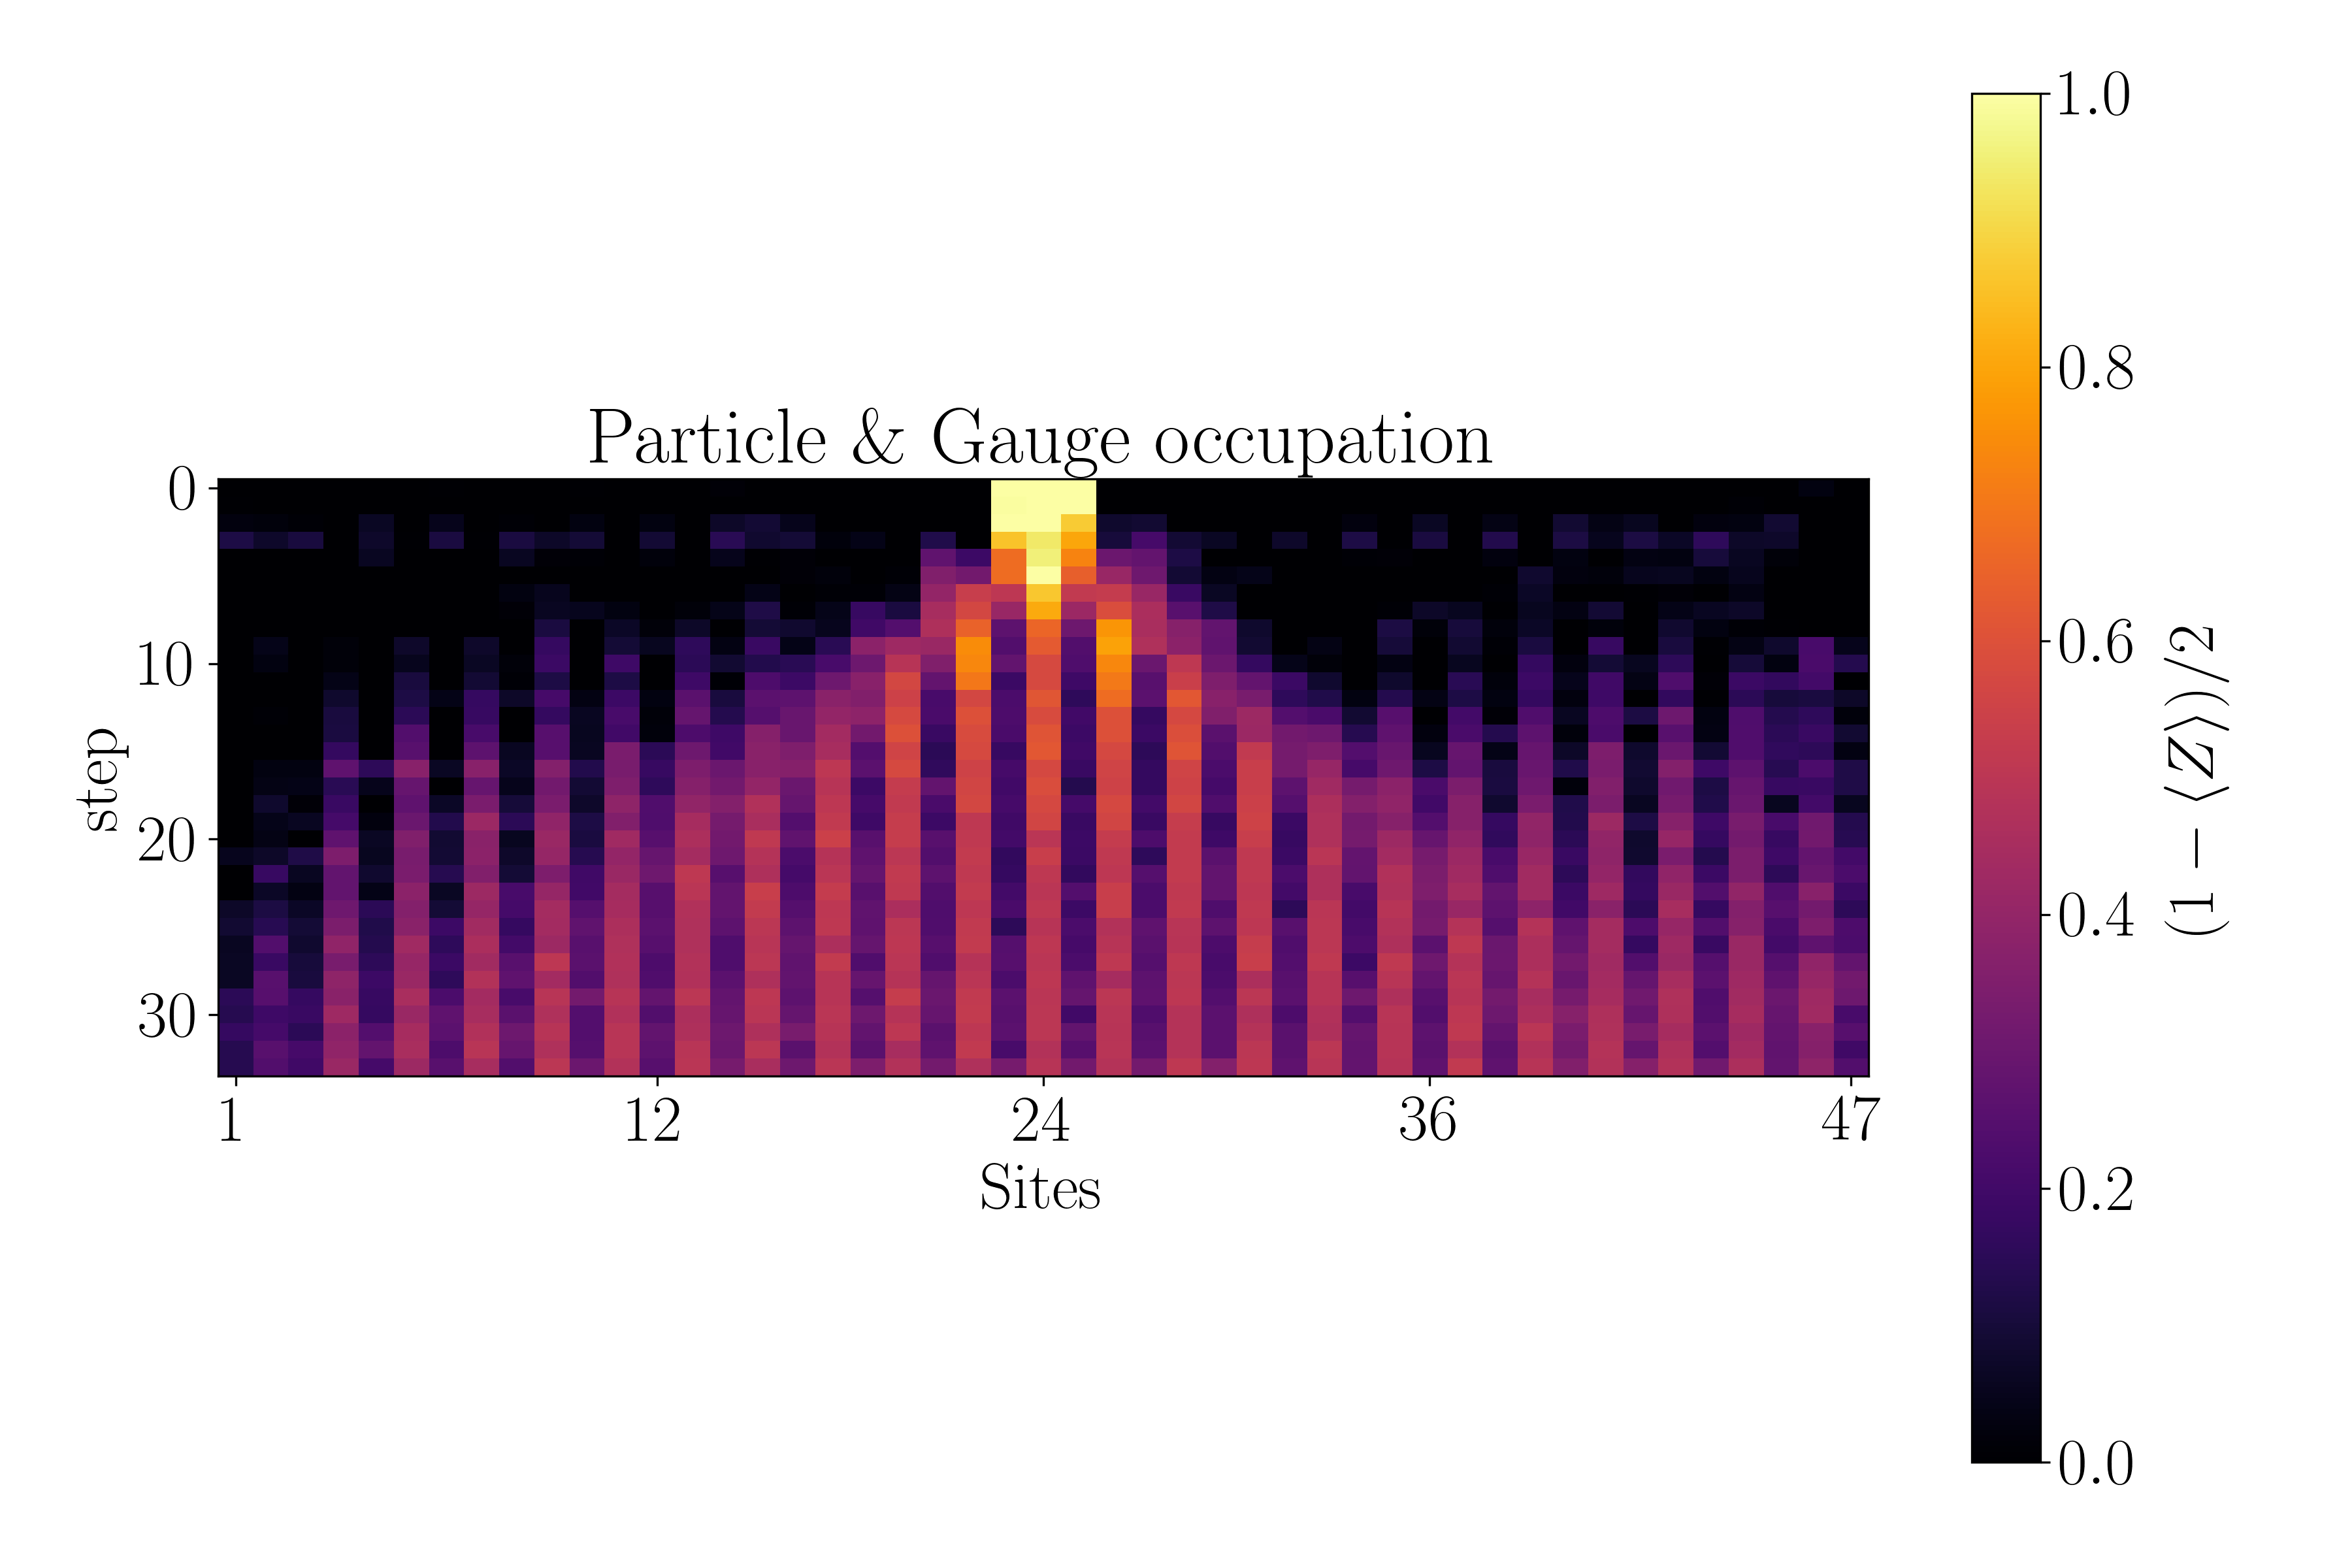
\includegraphics[width=\textwidth]{Results figs/hardware_z2pairquench_maxt_8_steps_35_L_24_J_1.0000_h_0.0500_lamb_0.7000_g_None_pp_11_pl_1_zne_True_linear_1-1.2-1.5_mm_True_dc_XY4_pt_True_xbasis_False.png}
        \caption{$L = 16$}
    \end{subfigure}
    \caption{Dynamics of the mean occupation of matter and gauge sites in two chains of different length.}
\end{figure}

\printbibliography

\end{document}